% % % % % % % % % % % % % % % % % % % % % % % % % % % % % % % % % %
%  Devolutiva — Fase 1: Imersão
%  Disciplina: Design Thinking (DE_233) — ETE Cícero Dias
%  Profa. Samara Silva  ·  Recife, 17 de junho de 2026
% % % % % % % % % % % % % % % % % % % % % % % % % % % % % % % % % %

\documentclass[
  sigconf,
  nonacm, % Remove o rodapé da ACM
  language=portuguese
]{acmart}

% ── Desliga rodapé ACM ──────────────────────────────────────
\settopmatter{printacmref=false}
\setcopyright{none}
\acmYear{2026}
\let\balance\relax

% ── Mata a página temporária da ACM (compilação única via API) ──
\makeatletter
\def\acm@addtemp@page{}
\makeatother

% ── Pacotes ─────────────────────────────────────────────────
\usepackage[portuguese]{babel}
\usepackage{microtype}
\usepackage{booktabs}
\usepackage{tabularx}
\usepackage{array}
\usepackage{colortbl}
\usepackage[dvipsnames,table]{xcolor}
\usepackage[inline]{enumitem}
\usepackage{graphicx}
\usepackage{adjustbox}
\usepackage{fancyhdr}
\usepackage{eso-pic} % Para a capa preencher toda a página sem gerar páginas em branco

% ── Ajuste contra quebras de texto ruins (Textos Cortados) ──
\tolerance=1000
\emergencystretch=1.5em

% ── Cores ───────────────────────────────────────────────────
\definecolor{cgood}{HTML}{1E6B3A}
\definecolor{cwarn}{HTML}{8B4500}
\definecolor{cred}{HTML}{C0392B}
\definecolor{cmuted}{HTML}{666666}
\definecolor{crow}{HTML}{F2EFEB}

% ── Colunas customizadas para tabela ────────────────────────
\newcolumntype{L}[1]{>{\raggedright\arraybackslash}p{#1}}
\newcolumntype{C}[1]{>{\centering\arraybackslash}p{#1}}

% ── Comando nota destacada ───────────────────────────────────
\newcommand{\notadestaque}[2]{%
  \noindent\textbf{Nota:}\enspace%
  {\large\bfseries\color{cred}#1\,/\,#2\,pts}%
}

% ── Comando label de status ──────────────────────────────────
\newcommand{\statusok}[1]{{\small\bfseries\color{cgood}#1}}
\newcommand{\statuswarn}[1]{{\small\bfseries\color{cwarn}#1}}

% ── Renomeações PT-BR ────────────────────────────────────────
\AtBeginDocument{%
  \renewcommand{\abstractname}{Resumo}
  \renewcommand{\figurename}{Figura}
  \renewcommand{\tablename}{Tabela}
}

% ────────────────────────────────────────────────────────────
\begin{document}

% ── CAPA ────────────────────────────────────────────────────
\thispagestyle{empty}
\AddToShipoutPictureBG*{%
  \AtPageLowerLeft{%
    \IfFileExists{capa-imersao.png}{%
      
\includegraphics[width=\paperwidth,height=\paperheight]{capa-imersao.png}%
    }{%
      \IfFileExists{../../capa-imersao.png}{%
        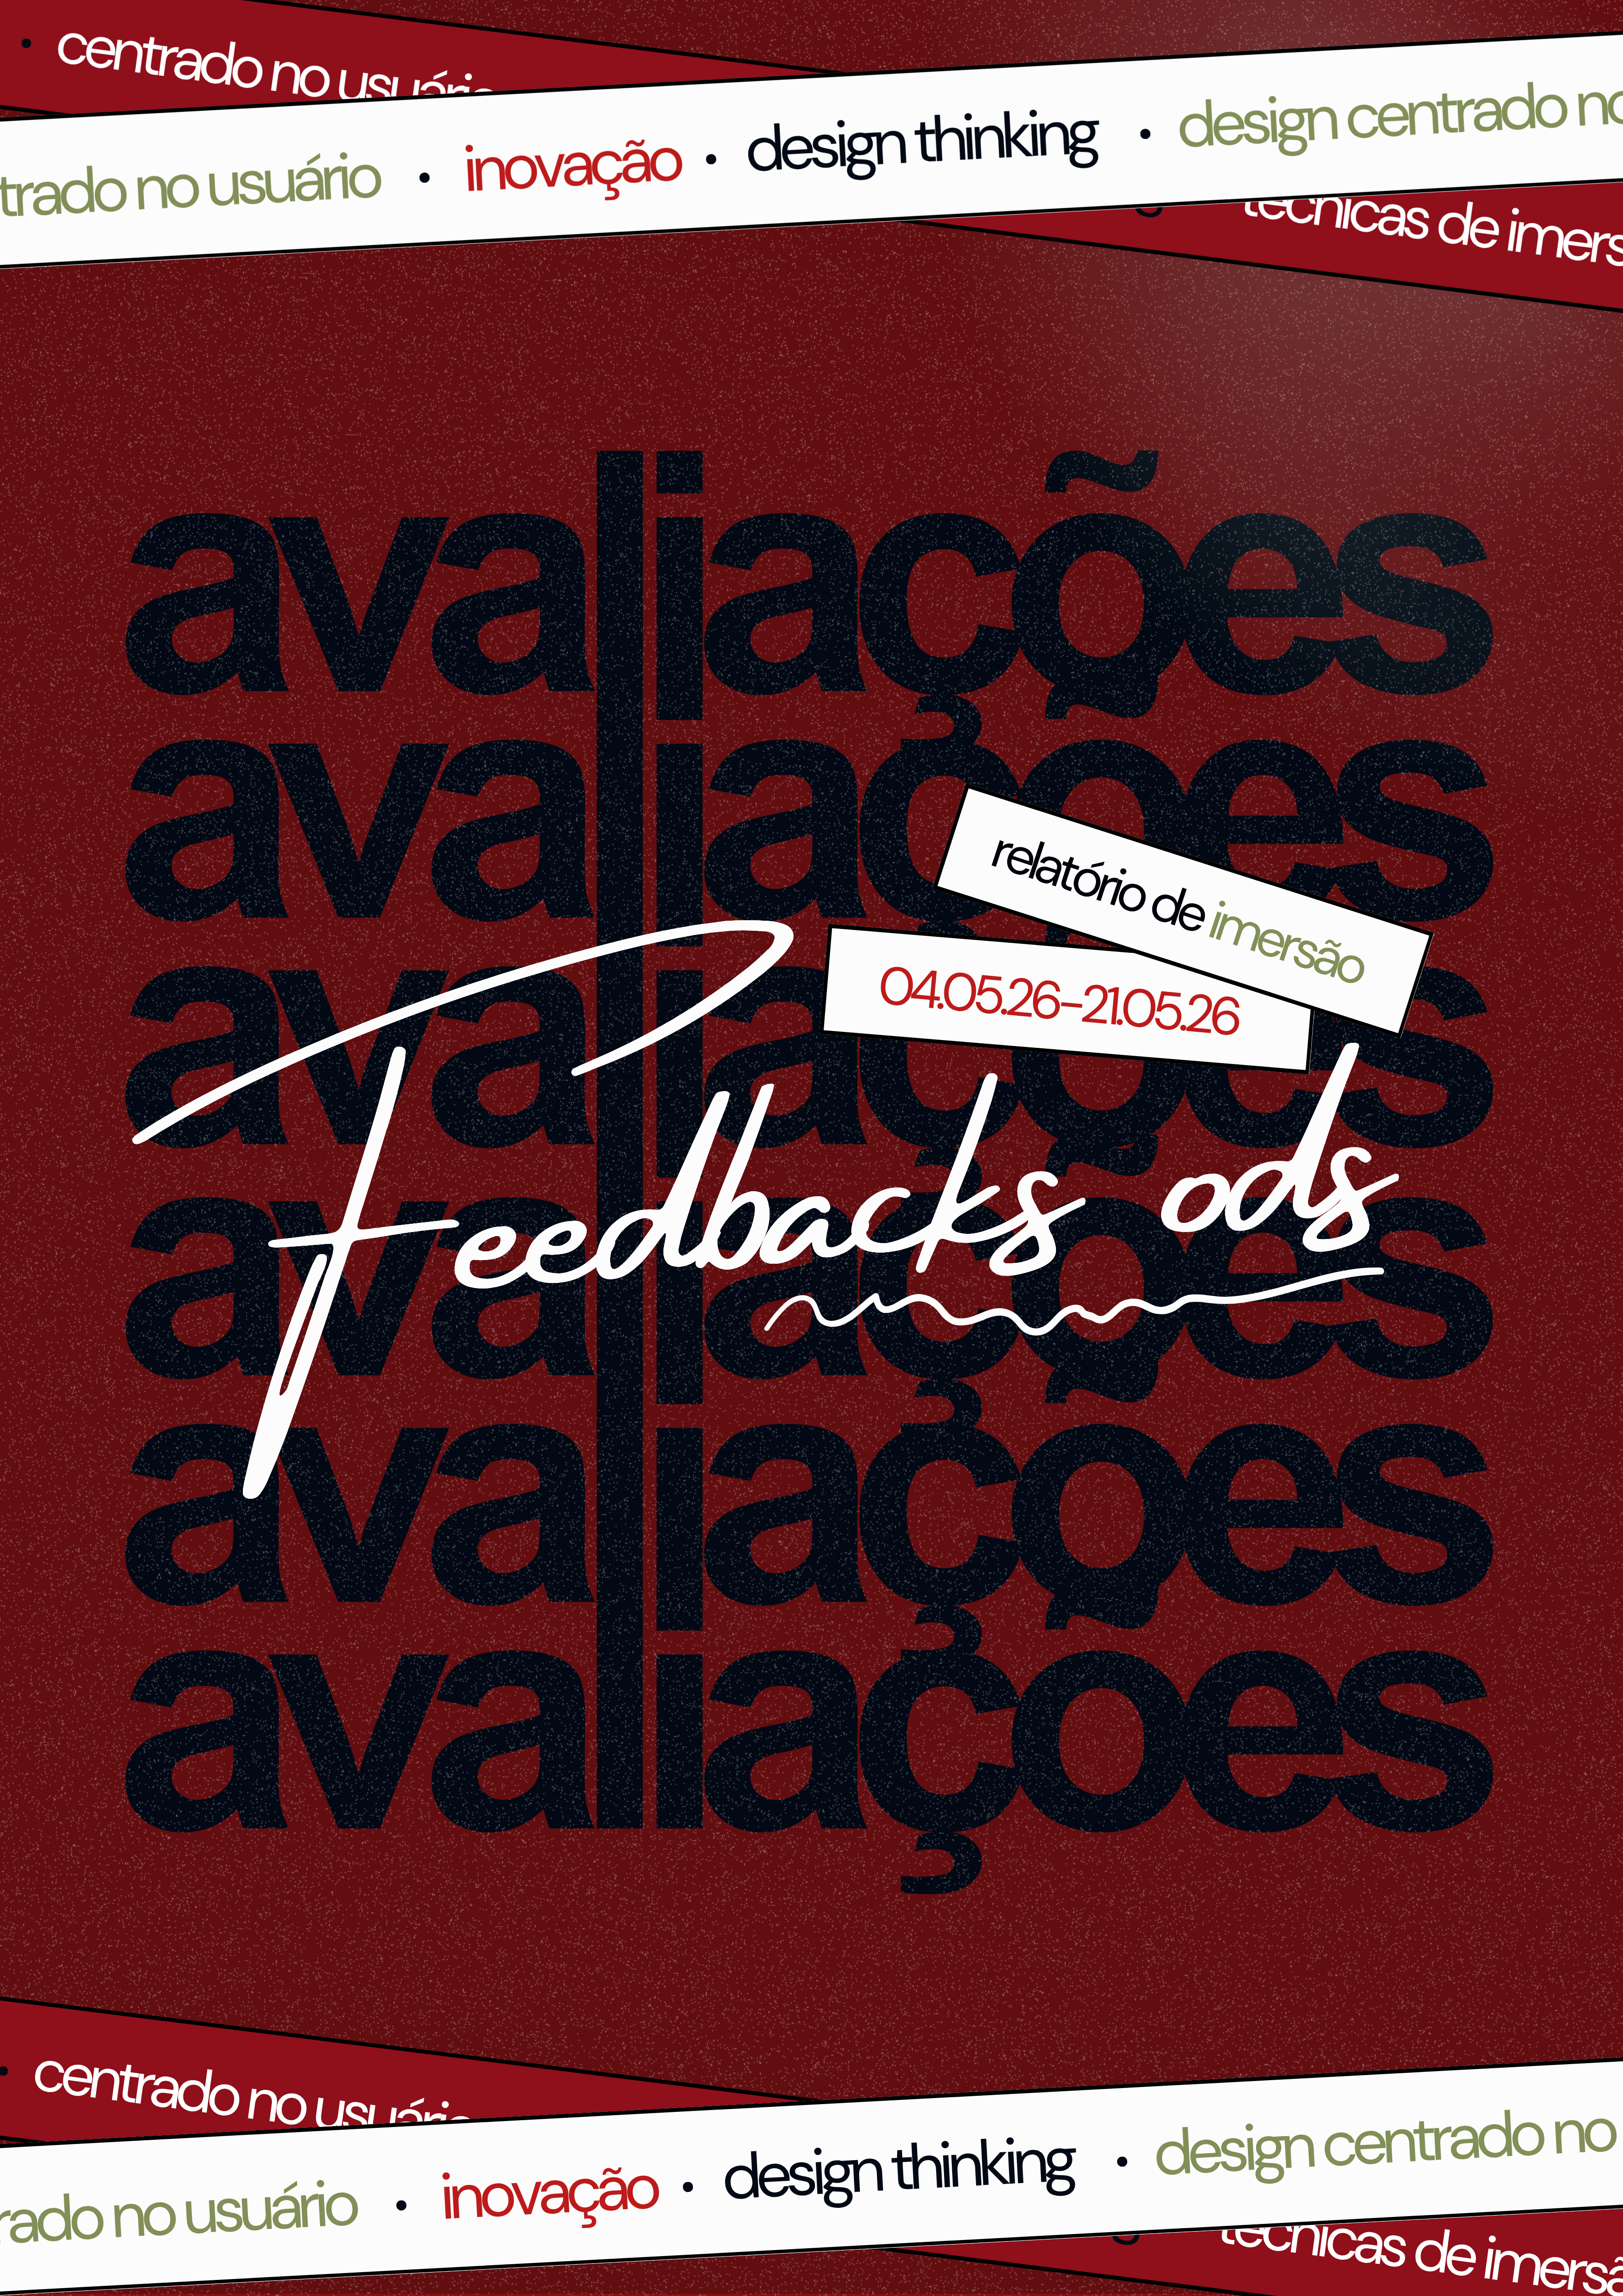
\includegraphics[width=\paperwidth,height=\paperheight]{../../capa-imersao.png}%
      }{%
        \parbox[b][\paperheight]{\paperwidth}{%
          \vspace*{10cm}\begin{center}{\large\color{gray}[capa-imersao.png não encontrada]}\end{center}%
        }%
      }%
    }%
  }%
}
\mbox{} % Caixa vazia para garantir que a página da capa seja gerada e preenchida
\clearpage

% ── CONFIGURAÇÃO DE PÁGINA PÓS-CAPA ─────────────────────────
\setcounter{page}{1}
\pagestyle{fancy}
\fancyhf{}
\renewcommand{\headrulewidth}{0pt}
\fancyfoot[C]{\thepage}
\setlength{\headsep}{0.8cm} % Distancia o cabeçalho do conteúdo das colunas

% ── METADADOS ────────────────────────────────────────────────
\title{Feedback Avaliativo de Projeto: Design Thinking --- Fase 1 — Imersão}

\author{Profa.\ Samara Silva}
\authornote{Grupo: \textbf{Grupo 01 - Fome Zero} \textperiodcentered\ Per\'{i}odo: 04-21 de maio de 2026 \textperiodcentered\ Avaliado em: 17 de junho de 2026.}
\email{samarasilvia.educa@gmail.com}
\affiliation{%
  \institution{ETE C\'{i}cero Dias}
  \department{M\'{o}dulo 1 --- Turma A · 2026.1}
  \city{Recife}
  \state{Pernambuco}
  \country{Brasil}
}

\author{Grupo 01 - Fome Zero}
\affiliation{%
  \institution{ETE C\'{i}cero Dias}
  \department{Turma --- Turma A · 2026.1}
  \city{Recife}
  \state{Pernambuco}
  \country{Brasil}
}
\maketitle

\vspace{1em}
\section{Avaliação Geral}

\notadestaque{2,27}{3,00}

A avaliação foi concluída. A seguir o resumo dos critérios e os comentários detalhados.

\subsection{Resumo dos Critérios}

\rowcolors{2}{crow}{white}
\begin{tabular}{@{} L{2.6cm} C{2.5cm} C{1.1cm} C{1.1cm} @{}}
\toprule
\textbf{Critério} & \textbf{Status} & \textbf{Nota} & \textbf{Máx.} \\
\midrule
Pesquisa Desk & \statusok{Completo} & \textbf{0,50} & 0,50 \\
Matriz de Alinhamento & \statusok{Completo} & \textbf{0,50} & 0,50 \\
Matriz CSD \& Perguntas de pesquisa & \statuswarn{Completo c/ ressalvas} & \textbf{0,42} & 0,50 \\
Pesquisa Primária & \statuswarn{Completo c/ ressalvas} & \textbf{0,85} & 1,50 \\
\midrule
\textbf{Total} & & \textbf{\color{cred}2,27} & \textbf{3,00} \\
\bottomrule
\end{tabular}

\section{Comentários por Critério}

\subsection{Pesquisa Desk}

\noindent\statusok{0,50\,/\,0,50 pts · Completo}

\begin{itemize}[leftmargin=14pt,itemsep=1pt,topsep=3pt,parsep=0pt]
  \item[\textcolor{cgood}{$\checkmark$}] {\small\textcolor{cgood}{Dados secundários relevantes e atuais sobre o ODS escolhido}}
  \item[\textcolor{cgood}{$\checkmark$}] {\small\textcolor{cgood}{Fontes confiáveis: ONU, IBGE, artigos acadêmicos ou jornalísticos}}
  \item[\textcolor{cgood}{$\checkmark$}] {\small\textcolor{cgood}{Contextualiza o problema com base factual}}
  \item[\textcolor{cgood}{$\checkmark$}] {\small\textcolor{cgood}{Conexão clara entre os dados e o problema}}
  \item[\textcolor{cgood}{$\checkmark$}] {\small\textcolor{cgood}{Coerência entre a CSD e o que foi pesquisado}}
  \item[\textcolor{cgood}{$\checkmark$}] {\small\textcolor{cgood}{Mínimo de 5 referências/links, esperado 8, ideal de 15 para cima}}
\end{itemize}

O grupo está de parabéns pela qualidade da Desk Research! A escolha das fontes demonstra muita maturidade. Vocês buscaram referências com altíssima credibilidade (FAO, IBGE, EMBRAPA, MAPA) e dados extremamente atualizados, o que traz um embasamento fantástico para justificar a importância do projeto. Senti falta de dados diferentes como artigos ou algo de teor acadêmico, mas não tira o mérito do trabalho.

\textit{\textbf{Seção presente no relatório}}

A redação desta seção está excelente! O texto é extremamente claro, bem fundamentado e utiliza uma linguagem técnica e acadêmica perfeitamente adequada ao rigor exigido pelo projeto. A forma como vocês dividiram as frentes estratégicas (Análise Documental, Quantitativa e Levantamento Bibliográfico) demonstra muita organização e maturidade metodológica.

Outro ponto fortíssimo do trabalho foi a consolidação das inferências no final do texto. Extrair os dados da pesquisa teórica e estruturá-los de forma quantitativa (Dado 1 a Dado 6) para a construção de gráficos foi uma excelente decisão. Isso não apenas facilita a leitura e a visualização do problema, mas também comprova a capacidade analítica da equipe em transformar textos densos em informações acionáveis que justificam a criação do aplicativo.

Ótimo trabalho de síntese e argumentação! Parabéns, fiquei muito feliz com o trabalho de vocês.

\subsection{Matriz de Alinhamento}

\noindent\statusok{0,50\,/\,0,50 pts · Completo}

\begin{itemize}[leftmargin=14pt,itemsep=1pt,topsep=3pt,parsep=0pt]
  \item[\textcolor{cgood}{$\checkmark$}] {\small\textcolor{cgood}{Identifica claramente quem é afetado pelo problema}}
  \item[\textcolor{cgood}{$\checkmark$}] {\small\textcolor{cgood}{Define o que o grupo pretende descobrir durante a imersão}}
  \item[\textcolor{cgood}{$\checkmark$}] {\small\textcolor{cgood}{As técnicas de imersão escolhidas são coerentes com os objetivos da pesquisa}}
  \item[\textcolor{cgood}{$\checkmark$}] {\small\textcolor{cgood}{Delimita adequadamente o que está dentro do escopo do projeto}}
  \item[\textcolor{cgood}{$\checkmark$}] {\small\textcolor{cgood}{Delimita adequadamente o que está fora do escopo do projeto}}
  \item[\textcolor{cgood}{$\checkmark$}] {\small\textcolor{cgood}{Apresenta uma hipótese inicial de solução relacionada ao problema investigado}}
  \item[\textcolor{cgood}{$\checkmark$}] {\small\textcolor{cgood}{Os resultados esperados da imersão são claros e coerentes com os objetivos da pesquisa}}
  \item[\textcolor{cgood}{$\checkmark$}] {\small\textcolor{cgood}{Há coerência entre os diferentes campos da matriz (problema, público, escopo, pesquisa e solução)}}
  \item[\textcolor{cgood}{$\checkmark$}] {\small\textcolor{cgood}{Preenchida com respostas, impressões ou perguntas reais do grupo sobre o problema}}
  \item[\textcolor{cgood}{$\checkmark$}] {\small\textcolor{cgood}{Linguagem clara e coerente, facilitando a compreensão das intenções do grupo}}
  \item[\textcolor{cgood}{$\checkmark$}] {\small\textcolor{cgood}{Serviu de base para planejar a pesquisa primária}}
\end{itemize}

Nada a declarar. Está tudo de acordo com o esperado!

\subsection{Matriz CSD \& Perguntas de pesquisa}

\noindent\statuswarn{0,42\,/\,0,50 pts · Completo c/ ressalvas}

\begin{itemize}[leftmargin=14pt,itemsep=1pt,topsep=3pt,parsep=0pt]
  \item[\textcolor{cgood}{$\checkmark$}] {\small\textcolor{cgood}{Os três quadrantes preenchidos: Certezas, Suposições, Dúvidas}}
  \item[\textcolor{cgood}{$\checkmark$}] {\small\textcolor{cgood}{Reflete o que o grupo sabe e precisa descobrir sobre o problema e seu contexto}}
  \item[\textcolor{cgood}{$\checkmark$}] {\small\textcolor{cgood}{Conteúdo específico do projeto — não genérico}}
  \item[\textcolor{cgood}{$\checkmark$}] {\small\textcolor{cgood}{Revela pensamento crítico}}
  \item[\textcolor{cgood}{$\checkmark$}] {\small\textcolor{cgood}{O quadrante de CERTEZAS expõe informações comprovadas ou confirmadas sobre o problema}}
  \item[\textcolor{cgood}{$\checkmark$}] {\small\textcolor{cgood}{Os itens do quadrante de CERTEZA estão relacionados diretamente ao contexto e ao público afetado}}
  \item[\textcolor{cgood}{$\checkmark$}] {\small\textcolor{cgood}{O quadrante de SUPOSIÇÕES expõe Informações que o grupo acha que são verdadeiras, mas ainda não comprovou}}
  \item[\textcolor{cgood}{$\checkmark$}] {\small\textcolor{cgood}{Os itens do quadrante de SUPOSIÇÃO demonstram reflexão sobre possíveis causas, comportamentos ou necessidades}}
  \item[\textcolor{cgood}{$\checkmark$}] {\small\textcolor{cgood}{O quadrante de DÚVIDAS expõem perguntas que o grupo precisa responder na pesquisa ou imersão como um todo}}
  \item[\textcolor{cgood}{$\checkmark$}] {\small\textcolor{cgood}{Os itens do quadrante de DÚVIDAS representam lacunas reais de conhecimento}}
  \item[\textcolor{cgood}{$\checkmark$}] {\small\textcolor{cgood}{O conteúdo da matriz está focado no problema investigado e não apenas no tema ou na ODS}}
  \item[$\square$] {\small\textcolor{cmuted}{Perguntas de Pesquisas formuladas como objetivos que norteiam o projeto geral}}
\end{itemize}

A equipe demonstrou um bom entendimento na construção da Matriz CSD, que é um excelente ponto de partida. A coluna de 'Dúvidas' está muito bem construída e contém pontos altamente estratégicos. Eu particularmente adorei que abrangeram vários escopos desde algo financeiro até logístico.

No entanto, há um desvio metodológico importante na etapa de planejamento das perguntas de pesquisa que precisa ser corrigido: \textbf{houve uma sobreposição entre as Perguntas de Pesquisa e o Roteiro/Formulário do usuário. }Para o rigor acadêmico e prático do Design de Serviços/Produtos, é fundamental distinguir estas três camadas:

\begin{itemize}[leftmargin=14pt,itemsep=2pt,topsep=4pt]
  \item \textbf{Dúvidas (Matriz CSD):} Representam as incertezas internas do grupo. É o levantamento bruto do que a equipe não sabe. ex:\textit{"Os estudantes preferem estudar pelo celular ou pelo notebook?"}
  \item \textit{"Eles ainda têm o costume de usar agenda de papel?"}
  \item \textit{"Quanto tempo eles conseguem focar antes de pegar o celular?"}
\end{itemize}

\begin{itemize}[leftmargin=14pt,itemsep=2pt,topsep=4pt]
  \item \textbf{Perguntas de Pesquisa:} São os objetivos da investigação. Elas guiam o \textit{projeto} e a \textit{equipe}, sintetizando as dúvidas e suposições da CSD em grandes eixos investigativos. \textbf{Essas perguntas não devem ser feitas diretamente ao usuário. }ex:\textit{"Quais são os principais métodos e ferramentas de organização utilizados por universitários hoje, e quais são os maiores gatilhos comportamentais de distração durante o estudo?"}
\end{itemize}

\begin{itemize}[leftmargin=14pt,itemsep=2pt,topsep=4pt]
  \item \textbf{Roteiro/Formulário de Pesquisa:} É o instrumento de coleta. Aqui, as perguntas de pesquisa são traduzidas para a linguagem do usuário, de forma conversacional e empática, para evitar vieses. ex:\textit{"Você poderia me contar como costuma se organizar quando tem uma semana cheia de provas?"}
  \item \textit{"Lembre da última vez que você sentou para estudar e acabou perdendo o foco. Como foi isso? O que acabou tirando a sua atenção?"}
\end{itemize}

\textbf{O impacto desse erro:} Em vez de definirem os eixos estratégicos que o projeto precisa investigar, a equipe inseriu as perguntas de interação direta com o usuário no lugar das Perguntas de Pesquisa. Ao fazer isso, o projeto perde o seu "norte" analítico.

Por exemplo: a questão que vocês listaram, \textit{"Sobre o descarte de alimentos na sua casa: Quando você prepara refeições, o que costuma fazer com as partes não convencionais dos vegetais e frutas (cascas, talos, folhas e sementes)?"}, é uma excelente pergunta de \textbf{Formulário/Roteiro} para fazer ao usuário. No entanto, a verdadeira \textbf{Pergunta de Pesquisa} (que deveria estar preenchendo essa seção do documento para guiar a equipe) deveria ser algo como: \textbf{"Quais são os hábitos atuais de descarte e o nível de aproveitamento integral dos alimentos na rotina doméstica do nosso público?"}

\textbf{Ação necessária:} Revisar o instrumento de pesquisa. Desdobrem as Perguntas de Pesquisa atuais em perguntas adequadas e táticas.

\subsection{Pesquisa Primária}

\noindent\statuswarn{0,85\,/\,1,50 pts · Completo c/ ressalvas}

\textit{\textbf{Seção presente no relatório}}

O texto que descreve os resultados da pesquisa está excelente. A redação é clara, objetiva e traz inferências muito ricas. A forma como vocês estruturaram os dados percentuais ao final (Dado Survey 1 ao 5) demonstra uma ótima capacidade de síntese. Vocês conseguiram cruzar as respostas para comprovar a viabilidade e a aceitação do aplicativo, o que atende perfeitamente ao objetivo desta etapa. Parabéns pela estruturação!

\textit{\textbf{InStrumento de coleta (Google forms)}}

Embora a estrutura básica do formulário esteja correta e os resultados tenham sido úteis, existem pontos importantes de melhoria para que a pesquisa alcance um rigor metodológico maior em projetos futuros:

\begin{enumerate}[leftmargin=14pt,itemsep=2pt,topsep=4pt]
  \item \textbf{Descrição e Termo de Consentimento:} A introdução do formulário foi muito breve. Faltou especificar que vocês são estudantes do curso de Desenvolvimento de Sistemas da ETE Cícero Dias, detalhar um pouco mais o propósito do projeto e, muito importante em formulários, informar o tempo estimado de resposta (ex: "Esta pesquisa leva apenas 2 minutos").
  \item \textbf{Perfil do Usuário (Dados Demográficos):} O formulário não coleta informações básicas de quem está respondendo. Mesmo sendo anônimo, é fundamental saber a faixa etária, a composição familiar (quantas pessoas moram na casa) e o contexto socioeconômico. Isso permite cruzar dados importantes (ex: "Será que famílias maiores desperdiçam mais?" ou "Qual a idade do público que mais aceita a tecnologia?").
  \item \textbf{Volume e Diversidade de Perguntas:} Um questionário com apenas 5 perguntas limita muito o aprofundamento do tema. O ideal para uma pesquisa desse porte seria entre 10 e 12 perguntas, preferencialmente divididas por seções (Ex: Seção 1 - Perfil; Seção 2 - Hábitos de Consumo; Seção 3 - Relação com Tecnologia).
  \item \textbf{Tipos de Resposta:} Houve uma limitação ao usar apenas perguntas de múltipla escolha (onde só se marca uma opção). Em pesquisas de campo, é enriquecedor incluir perguntas de "caixa de seleção" (onde o usuário pode marcar mais de um motivo) e, principalmente, perguntas abertas (texto curto ou longo) para captar opiniões espontâneas e insights qualitativos que a equipe não havia previsto.
\end{enumerate}

Apesar dessas oportunidades de melhoria no formulário, os dados coletados foram suficientes para embasar a justificativa do projeto nesta etapa. Excelente trabalho de análise!

\section{Considerações Finais}

Os ajustes indicados são de natureza metodológica e devem ser
incorporados para as próximas entregas.
Continuem assim.

% ── Assinatura ───────────────────────────────────────────────

\vspace{1.5em}
\noindent\rule{\linewidth}{0.4pt}

\begin{flushright}
\textbf{Profa.\ Samara Silva}\\
{\small\color{cmuted} Design Thinking --- DE\_233 · ETE Cícero Dias}\\
{\small\color{cmuted} Recife, 17 de junho de 2026}
\end{flushright}

% ── Sem referências bibliográficas ───────────────────────────

\appendix
\onecolumn
\section{Critérios e Níveis de Avaliação}

Esta seção apresenta os critérios de avaliação para referência dos estudantes.

\subsection{Níveis de Completude}

\begin{tabularx}{\linewidth}{@{} p{4cm} p{1.5cm} X @{}}
\toprule
\textbf{Nível} & \textbf{\%} & \textbf{Descrição} \\
\midrule
Completo & 100\% & Fez tudo e fez certo. Critério plenamente atendido. \\
Completo c/ ressalvas & 85\% & Fez tudo, mas algo ficou incorreto ou impreciso. Esforço total, qualidade com falha. \\
Completo, mas inadequado & 70\% & Preencheu todos os itens, porém boa parte do conteúdo não atende ao propósito da atividade. \\
Faltou pouco & 65\% & Fez bastante e acertou o que fez. Faltaram partes, mas o que entregou presta. \\
Faltou pouco c/ erros & 60\% & Fez bastante, mas errou partes relevantes. Metade do caminho com qualidade irregular. \\
Faltou muito & 40\% & Fez pouco, mas o que fez está correto. Entrega incompleta, execução ok. \\
Faltou muito e errou & 25\% & Fez pouco e ainda errou. Esforço baixo, qualidade baixa. \\
Errado & 10\% & Tentou, mas a abordagem foi incorreta por completo. Reconhece a tentativa. \\
Não fez & 0\% & Critério não entregue. \\
\bottomrule
\end{tabularx}

\vspace{1em}
\subsection{Penalizações por Atraso}

\begin{tabularx}{0.6\linewidth}{@{} X p{5cm} @{}}
\toprule
\textbf{Atraso} & \textbf{Desconto} \\
\midrule
Até 1 dia & -10\% \\
2–3 dias & -20\% \\
Mais de 3 dias & -30\% \\
Não entregou & Zera a nota \\
\bottomrule
\end{tabularx}

\section{Devolutiva Individual}

A nota individual é calculada aplicando o fator de contribuição sobre a nota do grupo em cada fase.

\subsection{Fatores de Contribuição}

\begin{tabularx}{0.6\linewidth}{@{} X c @{}}
\toprule
\textbf{Fator} & \textbf{Multiplicador} \\
\midrule
Liderou & 100\% \\
Participou & 100\% \\
Participou pouco & 70\% \\
Só fez sua parte & 40\% \\
Não participou & 0\% \\
\bottomrule
\end{tabularx}

\vspace{1em}
\subsection{Notas por Integrante}

\begin{tabularx}{\linewidth}{@{} X X p{2.5cm} @{}}
\toprule
\textbf{Integrante} & \textbf{\small DT Fase 1 — Imersão} & \textbf{Total} \\
\midrule
André da Silva Durães & 0,00 \textit{(Não participou)} & \textbf{0,00} \\
Bruna Maria do Nascimento Costa & 0,00 \textit{(Não participou)} & \textbf{0,00} \\
João Gabriel Cavalcanti & 2,27 \textit{(Participou)} & \textbf{2,27} \\
Suammyr Cavalcante do Carmo & 2,27 \textit{(Liderou)} & \textbf{2,27} \\
Maria Zilda Ferreira Pinto & 2,27 \textit{(Participou)} & \textbf{2,27} \\
Ayran Gabriel Duque Souza Lima & 0,00 \textit{(Não participou)} & \textbf{0,00} \\
\bottomrule
\end{tabularx}

\end{document}
